\subsubsection{Mutation}
\label{sec:bg:gp:variation:mutation}
  Mutation, another crucial genetic operator, introduces new genetic material 
  into the population, thus maintaining genetic diversity and preventing 
  premature convergence to suboptimal solutions.
  In the context of GP, the mutation operator modifies a program in the
  population, while ensuring the resultant individual's syntactic correctness.

  In tree-based GP, a common form of mutation is the \emph{point 
  mutation}~\autocite{poliFieldGuideGenetic2008a,wilhelmstotterJeneticsJavaGenetica},
  which selects a random node from an individual and replaces it with a random
  primitive with the same arity.
  This operator is similar to the bit-flip mutation operator used on 
  \vref{sec:bg:ga:var:mut}.
  As with bit-flip mutation, point mutation can also be applied with a certain
  probability to each node in an individual, meaning that more than one node
  can be mutated in a single individual.

  Suppose we mutate all the individuals in the population resulting from the
  crossover operation in \vref{sec:bg:gp:var:cx}, and that exactly
  one node is mutated in each individual.
  Let the selected nodes be \(\clubsuit = \sin\) in \(\mathbf{I}_2\),
  \(\spadesuit = 7\) in \(\mathbf{I}_3\), \(\heartsuit = 5\) in 
  \(\mathbf{O}_1\), and \(\diamondsuit = 2\) in \(\mathbf{O}_2\).
  Then, a possible result of applying the point mutation operator can be:

  \[
    M\!\left(
      \begin{bmatrix}
        I_2 \\ I_3 \\ O_1 \\ O_2
      \end{bmatrix}
    \right) = M\!\left(
      \begin{bmatrix}
        7 - (5 + \clubsuit(x)) \\
        \spadesuit + 2 \\
        \heartsuit \cdot 7 \\
        x^\diamondsuit - (5 + \sin(x))
      \end{bmatrix}
    \right) = \left(
      \begin{bmatrix}
        7 - (5 + \clubsuit'(x)) \\
        \spadesuit' + 2 \\
        \heartsuit' \cdot 7 \\
        x^{\diamondsuit'} - (5 + \sin(x))
      \end{bmatrix}
    \right) = \left(
      \begin{bmatrix}
        7 - (5 + \cos(x)) \\
        6 + 2 \\
        6 \cdot 7 \\
        x^3 - (5 + \sin(x))
      \end{bmatrix}
    \right)
  \]

  Here, \(\clubsuit'\), \(\spadesuit'\), \(\heartsuit'\), and \(\diamondsuit'\)
  are random primitives with the same arity as \(\clubsuit\), \(\spadesuit\),
  \(\heartsuit\), and \(\diamondsuit\), respectively.
  That being, \(\clubsuit' = \cos\), \(\spadesuit' = 6\), \(\heartsuit' = 6\),
  and \(\diamondsuit' = 3\).

  The fitness of the individuals in the population after applying the subtree 
  mutation operator is then evaluated.
  The results of this fitness evaluation are shown in 
  \vref{tab:bg:gp:var:mut:fitness}.
  A summary of the fitness of the population is presented in 
  \vref{tab:bg:gp:var:mut:fitness:summary}.

  \subimport{./}{tab-bg-gp-variation-mutation-node-fitness.tex}
  \subimport{./}{tab-bg-gp-variation-mutation-node-fitness-summary.tex}


  Just like the crossover operator, mutation can also significantly influence 
  the fitness and diversity of the population.
  By generating new structures in the population, mutation can help prevent
  stagnation and maintain diversity, thus avoiding premature convergence to
  suboptimal solutions.

  With this, we can conclude that after at the end of the generation, the
  population shows an improvement of 98.298\% in fitness, and 98.603\% in
  standard deviation.

  \[
    \frac{\bar{\Phi}_i - \bar{\Phi}_M}{\bar{\Phi}_i}
      = \frac{(44\,551.063\,525 - 758.472\,409)}{44\,551.063\,525} 
      \approx 98.298\%
  \]

  \[
    \frac{\sigma_i - \sigma_M}{\sigma_i}
      = \frac{(76\,814.062\,197 - 1\,073.402\,832)}{76\,814.062\,197}
      \approx 98.603\%
  \]

  \vref{fig:bg:gp:var:mut:pop} shows the population after applying the node
  mutation operator.
  Two points should be clear from this figure.
  First, all individuals of the population are closer to the target function
  than the individuals in the initial population.
  Second, the new fittest individual is \(\mathbf{O}_2\), this individual has a
  shape similar to the target function.

  \begin{figure}[ht!]
    \centering
    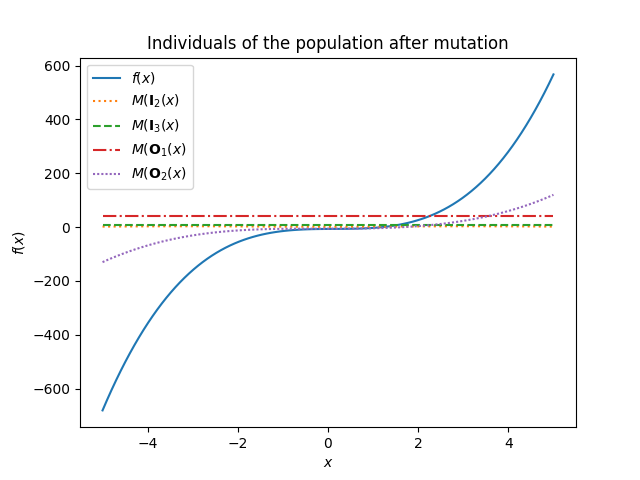
\includegraphics[width=0.8\textwidth]
      {img/theoretical_framework/gp_pop_mutated.png}
    \caption{Population after applying the node mutation operator}
    \label{fig:bg:gp:var:mut:pop}
  \end{figure}

  In summary, mutation plays a pivotal role in the genetic programming process.
  It injects fresh genetic material into the population, thereby promoting 
  diversity and ensuring the continual exploration of the search space.
  As demonstrated, mutation not only alters the structure of individuals but can 
  also lead to significant enhancements in fitness.
  By tactfully combining crossover and mutation operations, genetic programming 
  can efficiently traverse the vast landscape of possible solutions.
  This underscores the importance of maintaining a delicate balance between 
  exploration (introducing new genetic structures) and exploitation (refining 
  existing successful solutions).
